\documentclass[aspectratio=169]{beamer}

\usetheme[numbering=fraction]{metropolis} % clean layout
\metroset{progressbar=none}

% --- Layout: more whitespace and bigger readable text ---
\setbeamersize{text margin left=10mm, text margin right=10mm}
\linespread{1.05}

% Better list spacing
\usepackage{enumitem}
\setlist[itemize]{noitemsep, topsep=3pt, leftmargin=1.2em}
\setlist[description]{noitemsep, topsep=3pt}

% Make lists breathe (Metropolis can look cramped)
\setbeamertemplate{itemize/enumerate body begin}{\vspace{0.35em}}
\setbeamertemplate{itemize/enumerate body end}{\vspace{0.35em}}



\usepackage{graphicx}
\usepackage{booktabs}
\usepackage{ragged2e}

\setbeamertemplate{navigation symbols}{}
\setbeamerfont{title}{size=\LARGE}
\setbeamerfont{frametitle}{size=\Large}
\setbeamerfont{normal text}{size=\large}

% tighter, cleaner lists
\setlength{\parskip}{0.3em}
\setlength{\leftmargini}{1.2em}
\setbeamertemplate{itemize item}{\textbullet}


\usepackage[utf8]{inputenc}
\usepackage[T1]{fontenc}
\usepackage{graphicx}
\usepackage{tikz}
\usepackage{pgfgantt}
\usepackage[style=apa,backend=biber]{biblatex}

\addbibresource{mainbibliography.bib}

% Acronym definitions
\newcommand{\ac}[1]{\textsc{#1}}

% Title information
\title{CI/CD Observability in Containerized Environments}
\subtitle{Project Preparation (PREPD)}
\author{Eduardo Sousa}
\institute{Instituto Superior de Engenharia do Porto (ISEP)\\
Mestrado em Engenharia Informática\\
Cybersecurity and Systems Administration}
\date{\today}

\begin{document}

% Title slide
\begin{frame}
\titlepage
\end{frame}

\begin{frame}{Context and Motivation}
\begin{columns}[T,onlytextwidth]
  \column{0.55\textwidth}
  \begin{block}{Why it matters}
  \begin{itemize}
    \item \textbf{CI/CD services}: operational infrastructure
    \item \textbf{Failures}: block delivery and incident response
    \item \textbf{Diagnosis}: required across multiple services
  \end{itemize}
  \end{block}

  \column{0.42\textwidth}
  \begin{block}{Current reality}
  \begin{itemize}
    \item \textbf{Logs}: scattered across systems
    \item \textbf{Correlation}: weak across services
    \item \textbf{Decisions}: incomplete signals
  \end{itemize}
  \end{block}
\end{columns}
\end{frame}

\begin{frame}{Problem Statement}
\begin{columns}[T,onlytextwidth]
  \column{0.52\textwidth}
  \begin{block}{Technical constraints}
  \begin{itemize}
    \item \textbf{Non-privileged containers}: no host-level metrics
    \item \textbf{Telemetry fragmentation}: across CI/CD services
    \item \textbf{Mixed platforms}: Linux and Windows
  \end{itemize}
  \end{block}

  \column{0.46\textwidth}
  \begin{block}{Organizational constraints}
  \begin{itemize}
    \item \textbf{No host privileges}: administrative access denied
    \item \textbf{Security policy}: privileged containers forbidden
    \item \textbf{Diagnosis}: slow and manual on-prem
  \end{itemize}
  \end{block}
\end{columns}

\vspace{0.4em}
\textbf{Scope:} non-privileged containerized CI/CD on mixed OS
\end{frame}


% Slide 4: Research Gap
\begin{frame}{Research Gap}
\begin{columns}[T,onlytextwidth]
  \column{0.54\textwidth}
  \begin{block}{What the literature assumes}
  \begin{itemize}
    \item \textbf{Privileged access}: host or cloud-managed
    \item \textbf{Kernel mechanisms}: eBPF with elevated capabilities
    \item \textbf{Sidecar patterns}: Kubernetes contexts
  \end{itemize}
  \end{block}

  \column{0.44\textwidth}
  \begin{block}{Gap in practice}
  \begin{itemize}
    \item \textbf{Non-privileged}: mixed OS deployments
    \item \textbf{CI/CD workloads}: limited empirical guidance
    \item \textbf{Ephemeral tasks}: post hoc correlation underexplored
  \end{itemize}
  \end{block}
\end{columns}
\end{frame}

\begin{frame}{Objectives and Research Question}
\begin{block}{Central question}
  How can an \textbf{integrated observability framework} be designed and evaluated for
  \textbf{privilege-restricted CI/CD} environments?
\end{block}

\begin{block}{Objectives}
  \begin{itemize}
    \item \textbf{Architecture}: container-first without host privileges
    \item \textbf{Prototype}: reproducible images + deployment templates
    \item \textbf{Evaluation}: controlled fault injection + operational metrics
  \end{itemize}
\end{block}
\end{frame}

% Slide 6: Methodology Overview
\begin{frame}{Methodology Overview}
\textbf{Design Science Research Approach:}
\begin{description}
  \item[Phase 1] \textbf{Problem analysis} + PRISMA literature review
  \item[Phase 2] \textbf{Technology assessment} and tool selection
  \item[Phase 3] \textbf{Architecture} specification + prototype implementation
  \item[Phase 4] \textbf{Evaluation campaign} with controlled fault injection
  \item[Phase 5] \textbf{Analysis}, thesis writing, defense preparation
\end{description}

\vspace{0.3cm}
\textbf{Evaluation Strategy:}
\begin{itemize}
  \item \textbf{Quantitative}: MTTD, MTTR, resource overhead, throughput
  \item \textbf{Qualitative}: practitioner feedback via structured interviews
\end{itemize}
\end{frame}

% Slide 7: PRISMA Literature Review
\begin{frame}{PRISMA Literature Review}
\centering
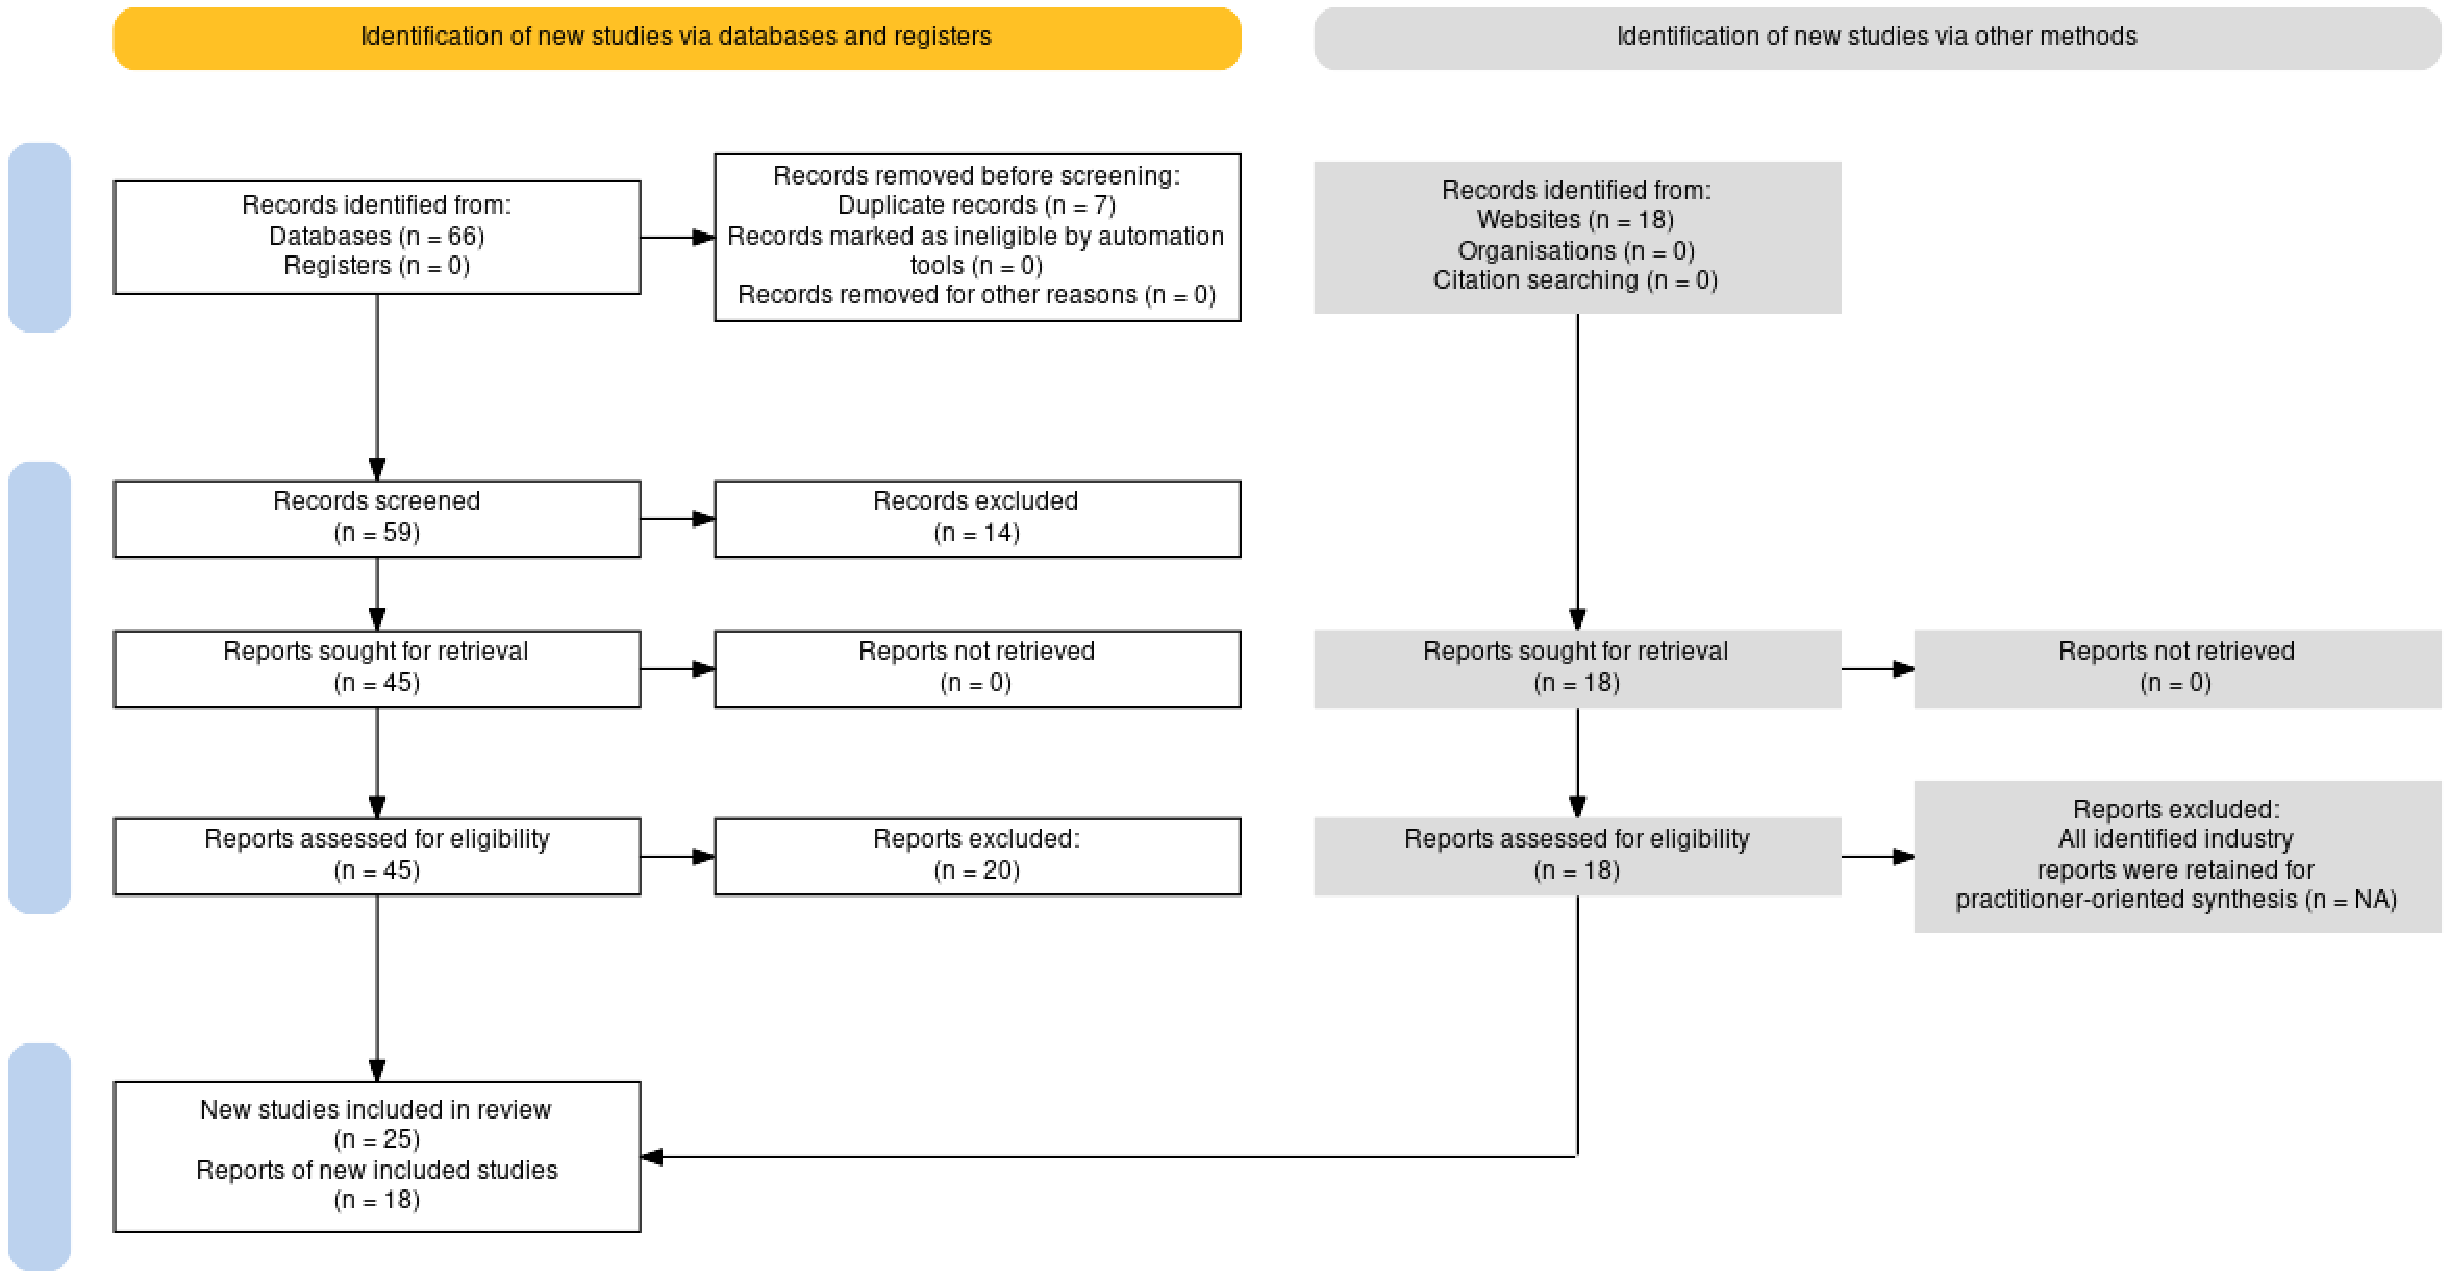
\includegraphics[height=0.78\textheight]{ch2_literature/assets/prisma.pdf} % or .png
\end{frame}

\begin{frame}{PRISMA Summary}
\vspace{1.0em}
\begin{center}
  \Large
  \begin{tabular}{@{}ll@{}}
    \textbf{66} & records identified (databases) \\
    \textbf{25} & peer-reviewed studies included \\
    \textbf{18} & industry sources retained \\
  \end{tabular}
\end{center}
\end{frame}




% Slide 9: Project Plan and Timeline
\begin{frame}{Project Plan and Timeline}
\begin{figure}
  \centering
  \footnotesize
  \begin{ganttchart}[
    hgrid,
    vgrid,
    x unit=0.28cm,
    y unit chart=0.48cm,
    bar height=0.48,
    group height=0.6,
    milestone height=0.5,
    milestone label font=\tiny,
    bar label font=\tiny,
    group label font=\tiny,
  ]{1}{26}

  \gantttitle{2026}{26}\\
  \gantttitle{Jan}{4}\gantttitle{Feb}{4}\gantttitle{Mar}{5}\gantttitle{Apr}{4}\gantttitle{May}{5}\gantttitle{Jun}{4}\\

  \ganttgroup{Project execution}{1}{26}\\

  \ganttbar[name=p1]{P1: Setup and planning}{1}{4}\\
  \ganttbar[name=p2]{P2: Tooling assessment}{3}{8}\\
  \ganttbar[name=p3]{P3: Architecture and prototype}{5}{13}\\
  \ganttbar[name=p4]{P4: Evaluation campaign}{14}{22}\\
  \ganttbar[name=p5]{P5: Analysis and writing}{19}{26}\\

  \ganttmilestone[name=m1]{M1: Tech selection}{4}\\
  \ganttmilestone[name=m2]{M2: Prototype deployed}{11}\\
  \ganttmilestone[name=m3]{M3: Eval protocol}{17}\\
  \ganttmilestone[name=m4]{M4: Measurements}{22}\\
  \ganttmilestone[name=m5]{M5: Submission}{25}

  \end{ganttchart}
  \caption{Project schedule (January--June 2026)}
\end{figure}
\end{frame}

% Slide 10: Summary and Next Steps
\begin{frame}{Summary and Next Steps}
\begin{columns}[T,onlytextwidth]
  \column{0.50\textwidth}
  \begin{block}{Established}
  \begin{itemize}
    \item \textbf{Problem framing}: privilege-restricted CI/CD
    \item \textbf{PRISMA review}: gaps identified
    \item \textbf{Methodology}: execution plan defined
  \end{itemize}
  \end{block}

  \column{0.50\textwidth}
  \begin{block}{Next phase}
  \begin{itemize}
    \item \textbf{Technology selection}: constraint-driven
    \item \textbf{Prototype}: architecture + implementation
    \item \textbf{Evaluation}: controlled fault injection
    \item \textbf{Validation}: practitioner feedback
  \end{itemize}
  \end{block}
\end{columns}
\end{frame}

% Final slide
\begin{frame}[plain]
\centering
\vfill
{\Huge Thank You}

\vspace{1.5em}

{\Large Questions?}

\vfill

\begin{center}
\small
Eduardo Sousa\\
\texttt{1200920@isep.ipp.pt}
\end{center}
\end{frame}

\end{document}
